\documentclass[12pt]{article}
\usepackage[english]{babel}
\usepackage[utf8]{inputenc}
\usepackage{graphicx}
\usepackage{float}
\usepackage[margin=1in]{geometry}
\title{CR1}
\author{Benoit Viguier}
\date{11/10/2014}
\begin{document}
\maketitle
\section{State of Art on MCTS}

In 1997, Deep Blue a computer built by IBM won a six games match against the current chess world champion Garry Kasparov. Human got beaten on Chess, but remain undefeated on Go, therefore the research is switching to that game. Until 2002, methods based on decompositions and positions evaluations were used in order to solve such games. Between 2002 and 2005 the Monte Carlo algorithm was used in order to find the best moves. Since 2006, it's implementation in a tree (MCTS) has been developped, skyrocketing the results in term of Artificial Intelligence on Go.
\begin{figure}[H]
\centering
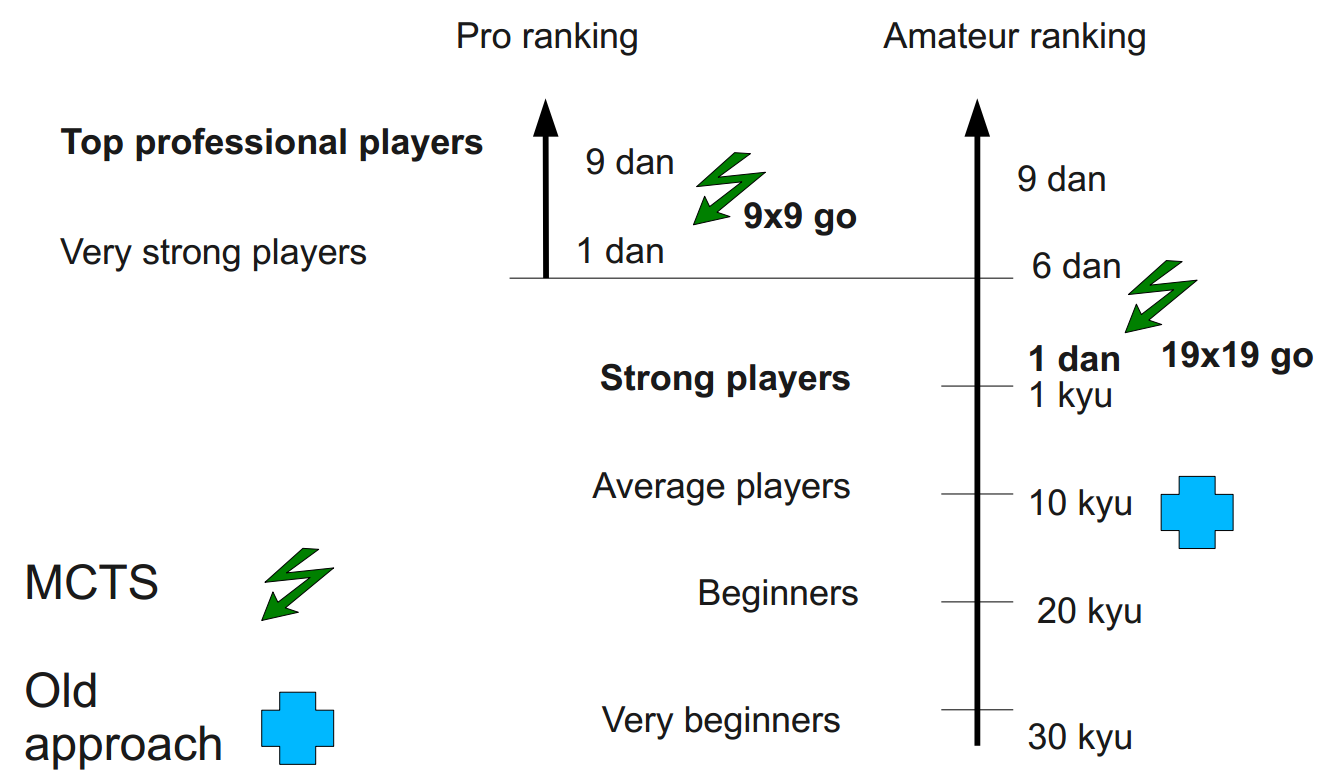
\includegraphics[width=15cm]{img/ranking.png}
\caption{\label{fig:ranking}Comparison between Go algorithm by ranking against human skill.}
\end{figure}
However MCTS wasn't the first method applied in order to solve Arimaa, the \ensuremath{\alpha\beta} method was used first. At the moment the top programms (Bomb by David Fotland : 2002 to 2008, Clueless by Jeff Bacher 2009) are ranked about 1800 elo. For comparison, strongest human players are rated around 2450 elo. But considering the promising results on the game of Go, it is highly plausible that the next top programms will be implemented with the MCTS.
\end{document}